\documentclass[a4paper]{article}
%\documentclass[sfsidenotes,symmetric]{tufte-book}
\usepackage{localstyle} % local style file

\title{Using Authorization Logics To Model Security Decisions in Mobile
  Systems\\\vspace{1em}Thesis Proposal}
\author{Joseph~Hallett}
\date\today

\bibliographystyle{plainnat}
\begin{document}
\maketitle
\setcounter{tocdepth}{3}
\tableofcontents
\pagebreak

\section{Introduction}

When an app is installed on Android it prompts the user to accept a list of
privileges granted to the app.  The user makes the decision based on what they
know about the app and their own security policies.  In practice a large number
of users accept the permissions whatever.  This is problematic because some apps
are over privileged\cite{Felt:2011kj} and some are malicious\cite{Zhou:2012cf}.
Other apps are considered to be \ac{PUS} because though they are not malicious
in themselves they handle data in a way that is not in the user's interests.

More generally users and computers make decisions, whether it update an app;
whether to connect to a website, based on security policies and trust
relationships.  These security policies may include the use of tools or experts
to decide whether something is malicious.  For instance a user may trust a
firewall program to enforce their network policy; and they may trust a tool like
\emph{Shorewall} to generate the actual policy for them.  Alternately a user
might wish to be able to install apps but only trust apps \emph{Amazon} have
vetted to be installed on their device.  \emph{The aim of this project is to
  formalize these security policies so they can be studied and enforced
  automatically.}

Mobile operating systems are similar to existing systems but come with a
different trust model and are used in a different manner.  Software is
downloaded from app stores, Apps run within sandboxes and must collaborate and
collude to share data with other apps. These devices contain more personal data
than ever before: sensors tracking users' locations,  gyroscopes measuring how
users move, and microphones listening to users calls.  The \ac{BYOD} movement
empowers users to take the devices they have at home and bring them into work.
This creates a tension between how the corporate IT department may require
employees to use their devices and the user's policies on how they want to use
their devices.  These features add a novel challenge to modelling these devices
and the stores and users surrounding them.  

Formalizing the policies allows comparisons to be made between different systems
and users.  When comparisons are made between the two biggest mobile OSs,
iOS~and~Android, the comparisons is informal: we say iOS is more closed, more of
a \emph{walled garden}, Android is more permissive.  With a formal language to
describe system policy we can make a precise comparison.  It allows us to 

There is decades of research on analysis tools.  These tools can infer complex
security properties about the code and systems they analyze.  What there is
missing is a glue layer between the assurances these tools can give and the
policies users are trying to enforce.  By using an \emph{authorization logic} as
the glue layer we can enforce the policy by building on the work on access
control in distributed systems.  Our static analysis tools can be trusted to
give statements about code, with other principles, that can be combined to
implement a security policy.


\section{Project description}

The aim of the thesis is to show how authorization logics can be used to make
security decisions in mobile devices.  Currently security decisions are made
manually by smart phone users and it is our belief that by automating these
choices users can avoid having to make security decisions and their overall
security be improved.  To do this we plan to look at the following areas: 

\begin{itemize}

  \item \emph{To instantiate a logic of authorization that allows us to model
      the trust relationships between the components of an operating system and
      the users.}  This will include analysis tools as principals and allow
    making decisions based on signed statements from them.  The logic must be
    able to model what happens when apps can collude.  The logic may be based
    off of earlier work on the \emph{SecPAL~language}\cite{Becker:2006vh} that
    was used for distributed access control decisions.

  \item \emph{To explore how security policies change with time and when apps
      can collude.}  A user's security policy need not be static.  People change
    jobs and may bring old devices to new environments requiring new security
    policies.  Apps can collude: two apps might meet a security policy when
    considered on their own but together they might act to share data
    inappropriately.  Over time an app might want greater access and increased
    permissions to support new functionality.  It is not obvious how to write
    and check security policies written in SecPAL for these scenarios and how
    to enforce the policy at runtime.

  \item \emph{To implement an app store that serves users only the apps that
      meet their security policies.}  This will include a user-study where we
    evaluate how well users comprehend their policies and the decisions made for
    them. This may lead into generating proof-carrying code certificates for
    apps that allow a device to check that their policy was met without having
    to do the full inference themselves.

  \item \emph{To model the decisions and trust relationships inherent in Android
      and other mobile operating systems.}  This will allow us to write a
    security policy that describes the current state in these systems and serve
    as a base to compare other systems against. 

  \item \emph{To study how users understand their security policies and the
      ways these policies are enforced.}  One of the advantages of SecPAL is
    that it is more readable compared to other authorization logics and access
    control languages.  Whilst end-users might not want to write their own
    policies they should be able to comprehend what a policy means, and they
    should be able to understand why their policy allows some decisions and not
    others.

\end{itemize}

\subsection{A Logic of Authorization For Mobile Devices}


\subsection{Compositional Policies Over Time}

Consider the case where a user has a smart phone and they are buying apps.  The
user must decide if they want to install an app: to do this they apply a series
of judgements called their \emph{security policy}.  

Whilst the user has their own security policy they apply they also have other
security policies they implicitly follow.  If they are downloading apps from an
app store they are also subject to the security policy of the app store and what
it is willing to sell.  If the phone runs in a corporate environment then they
may also be subject to the company's corporate policy.  Finally the operating
system itself may have certain restrictions on what it will allow: for example
the APK app format used on Android can also be installed on Blackberry, and Mer
operating systems.  Each of these systems may add additional restrictions that
may make some apps not installable.  An example of how this kind of policy might
be written is shown in Figure~\ref{example:composition}.

\begin{marginfigure}\label{example:composition}
  \begin{lstlisting}[language=SecPAL]
Phone says app is-installable
  if app meets UserSecurityPolicy,
     app meets AppStorePolicy,
     app meets ITDeptPolicy,
     app meets OSPolicy.

Phone says User can-say inf
  app meets UserSecurityPolicy.

Phone says PlayStore can-say 0
  app meets AppStorePolicy.

Phone says ITAdmin can-say inf
  app meets ITDeptPolicy.
  \end{lstlisting}
  \caption{A compositional security policy where an installation policy for a
    phone is dependent on other security policies.}
\end{marginfigure}
     
The phone might use this policy for a while, but then the user changes jobs.
Now they have to meet a new \code{ITDeptPolicy} set by a different administrator.
Should any installed apps be uninstalled if they don't meet the new policy?  If
we already have a certificate showing the apps passed the old policy can we
reuse it to create a new certificate that shows the app meets any additional
restrictions?

Whilst other authorization logics have looked at making one-time decisions about
whether to allow a computer to make a decision; there has been less work on
modelling these policies over time and seeing how a changing security policy
affects a changing device.  This could add novelty.

Alternatively say there is an app which the developer is continually improving
and adding new features.  When the app is installed it may meet the security
policy but with increasing features requiring access to more permissions and
introducing more complexity or a change of advert library the app no longer
meets the security policy.

Should the app be removed?  If the app is used every day by then the user may
not be pleased that the phone has decided to break their favorite
app\footnote{Though anecdotal evidence would suggest users tend to blame apps
  for failing rather than the frameworks they apps rely on; regardless of who is
  really to blame.}; equally just stopping updates for the app increases app
version fragmentation and reduces security by rejecting bug fixes.  Allowing the
update isn't correct either as it allows a means to break the security policy.

Whilst there have been several papers looking at (and proposing methods to stop)
excessive permissions in applications\cite{Felt:2011kj}\cite{Vidas:2011wr} there
has not been a thorough review of how permissions change for apps over time
and between versions of the same app. 

% TODO ADD BIT EXPLAINING HOW TO DO THIS


\subsection{Personally Curated App Stores}

The primary method of software distribution on mobile devices is through an app
store.  On iOS users have the \emph{App Store}: a curated market place run by
Apple (though other, albeit clunkier, distribution mechanisms do exist for even
non-jailbroken phones) that is perceived as being picky about the apps it sells.

On Android users have a far greater choice of marketplace.  The \emph{Play
  Store} is the standard app store distributed by Google and is less moderated
than Apple's store.  Amazon have their own app store that serves as a more
curated version of Google's offering and the default on their Kindle tablets.
Other app stores target specific regions: such as \emph{gFan} in China, and the
\emph{SK~T-Store} in Korea.  Some, such as \emph{Yandex.Store, AppsLib and
  SlideMe}, are pre-installed by OEMS who can't or don't want to meet Google's
requirements for the PlayStore.  The \emph{F-Droid} store only delivers open
source apps. Others exist to distribute pirated apps.  On average eight
percent\cite{AQUILINO:2013wr} of the apps in each of these alternative market
places is malware. The Play Store contains very little malware however (0.1\% of
total apps), whilst a third of the app in the Android159 store were found to be
malicious.

Each of these app stores have a different security policy.  They enforce these
policies when they pick which apps to sell to their users.  By using an
authorization logic to decide whether apps will meet a security policy we have
the ability to create a new kind of app store where offerings are tailored to
the user's security policy.  By creating app stores tailored to a security
policy we also give ourselves a way to empirically measure how restrictive a
security policy is: we can measure the number of apps offered inside the stores.

To enhance the trust in the store by the user digital evidence could be offered
with the app which would give devices a practical means to check that the app is
supported by their security policy without having to re-run all the checks
themselves; this should also save device battery life.  Proof-carrying
authentication\cite{Appel:1999dq} and authorization logics such as
BLF\cite{Whitehead:2004bu} have already introduced ideas from proof-carrying
code into authorization logics. The focus of this work, however, has been on
access control where a user is providing a proof that they have the credentials
to access a resource.   In the scenario we propose the role of the user is
reversed: the store offers many proofs to the user to increase their trust in
its wares; rather than the user offering one specific proof to prove they have
the right to complete a certain action.

\section{Review of Android Security}

Android is a Linux-based operating system designed for mobile phones and
increasingly used in consumer electronics. It comes with a large software
market that distributes apps. These apps are built on top of a virtual machine,
called Dalvik, and run within a sandbox provided by the OS that is based on
Linux's permissions model\cite{Drake:2014uq}.

\subsection{Permissions and Apps}

On top of the traditional permissions level Android has API permissions that
apps must request at install time. API permissions control access to
functionality such as the internet, reading or writing external storage, or to
learn about the state of the phone. These permissions are displayed to users at
install time and must be accepted if the app is to be installed. Most users do
not pay attention to these permissions and okay them no matter what is asked
for\cite{Felt:2012hm}. This has led to malware and \ac{PUS} that requests
excess permissions; which leads to apps sending premium text messages (a common
monetization strategy\cite{Chien:2011vw}) or stealing private information.

There are tools, however, which can detect when an app is over privileged. The
\emph{Stowaway} tool\cite{Felt:2011kj} mapped Android permissions onto the API
calls to access the functionality they enabled. This allowed them to detect
when apps were over privileged by looking for apps which had the permissions but
none of the associated API calls. The \emph{PScout} tool\cite{Au:2012ju}
improved upon Stowaway by increasing the accuracy of the permissions map and by
deriving the map from the Android source code, rather than the fuzzing based
methods Stowaway used.

\begin{marginfigure}\label{img:brightestflashlight}
  \centering
  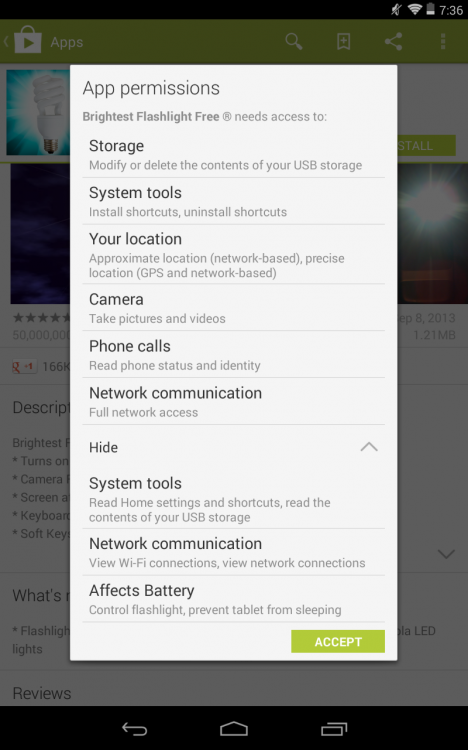
\includegraphics[width=0.8\textwidth]{img/brightestflashlight.png}
  \caption{The \emph{Brightest Flashlight Free} app prompting for it's permissions
    at install time. This app is over privileged as a flashlight app should have
    no need for GPS or phone data, or network access.}
\end{marginfigure}

One criticism of the API permissions is that they are quite broad. For instance
the \emph{internet} permission allows an app to send or receive anything on the
internet. Several people have proposed a \emph{fine grained permissions model}
and developed tools to support it. The \emph{RefineDroid, Dr.~Android \&
  Mr.~Hyde} tools\cite{Jeon:2012ki} are a suite designed to discover which
permissions can be made fine-grained, rewrite apps to use these permissions and
then enforce them at runtime; they do this on a stock Android system without
requiring rooting or kernel modification. Alternately the \emph{AppFence}
tool\cite{Hornyack:2011wq} works without modifying apps. It allows users to
write fine grained policies for what data an app can receive: if an app exceeds
its bounds then the request is either denied or fake data supplied in its place.
This does require modifications to the Android OS however. The \emph{AppGuard}
tool\cite{Backes:2013ec} offers something in between: it rewrites apps to use a
security monitor to enforce security policies at runtime.


\subsection{Intents and Collusion}

Android uses a novel IPC mechanism called \emph{Binder}. Apps use
\emph{intents} to share data and handle events. For instance if an app wishes
to handle an \code{SMS_RECEIVED} action it can declare itself a \emph{broadcast
  receiver} for it and the app will be started when the event occurs.
Alternatively if an app wants to open a URL in the browser it can send an
\code{ACTION_VIEW} intent and the user's chosen browser will take open the
URL.\@ Apps can create their own intents and can restrict usage of them (if they
wish) to only a limited number of other apps (or those signed with a specific
key).

These mechanisms also allow apps to collude to increase their privilege levels,
or share data inappropriately. To do this consider the case where there are two
apps communicating: one which can use the network and another which cannot. If
the unprivileged app asks the privileged app to send data on its behalf, and the
privileged app forwards the network responses back to it; then the unprivileged
app has the network permission without needing to declare it to the user.
Alternately if a privileged app does not secure its intents then they may break
the protections offered by permissions. An example of this was the \emph{Kies}
app on Samsung~Galaxy~S3 phones that could be exploited to allow any app to
install other apps\cite{moulu:8btkPowj}.

Several tools have been developed to detect these privilege escalation attacks
such as \emph{Quire}\cite{Bugiel:2012ui} that added origin tracing to intents.
Other tools such as \emph{ScanDroid}\cite{Fuchs:2009vi} statically analyze apps
to find data-flows across components and produce a series of constraints that
should be satisfied to guarantee information security. The
\emph{Kirin}\cite{Enck:2009ko} tool certifies apps at install time against a
policy based on the potential data-flows introduced by the permissions they
request.

The \emph{TaintDroid}\cite{Enck:2010uw} and \emph{FlowDroid}\cite{Fritz:2013vi}
have both had a large impact. Both tools both use taint analysis to track the
data passed between apps and detect when sensitive data is being leaked to an
app that should not have access to it through intents, however others have shown
that the approach is not perfect\cite{Sarwar:2013ta} and can be defeated by
malicious apps.

% TODO: INCLUDE SECTION ON ANDROID ROMS AND MALWARE

\section{Review of Policy Languages}

\subsection{Logics of Authorization}

When an action is performed, such as reading a file or installing an app, there
are a set of conditions that must be met for the action to go ahead. These
conditions form the \emph{authorization~policy} for that decision. When these
policies describe what actions are permissible in order to maintain a secure
system then we call it the \emph{security~policy}.

The policies often contain a notion of \emph{trust} where certain principals
may be trusted to make statements about other principals and what is
permissible. To model the relationships many logics have been proposed that can
be implemented to decide whether an action can be authorized automatically.

Early authorization logics, such as \emph{PolicyMaker}\cite{Blaze:dj} grew out
of the logics of authentication proposed by
\citeauthor*{Wobber:1994dh}\cite{Lampson:1992jg}\cite{Wobber:1994dh}.
PolicyMaker allowed authorities to declare trust in other principles (identified
through asymmetric keys) for certain actions or to declare further trust
relationships. The language was designed to be minimal and did not specify how
the policies should be checked: they suggested by using regular expressions, or
checking programs written in a sandboxed version of AWK however any language
could have been used. The author suggested that the language might be good as a
model for the public-key infrastructure. Later work introduced
\emph{KeyNote}\cite{Blaze:1999fa} which they claimed was a simplified version of
PolicyMaker designed to support public-key infrastructure.

Later other languages such as \emph{RT}\cite{Li:2002if} were introduced. RT
allowed principals to be given roles (in a manner similar to an \ac{RBAC}
access-control system) and for decisions to be made based on which roles an
entity held. This meant that RT could express general statements that were not
expressible in the PolicyMaker languages such as:
\begin{quote}
  ``Anyone who is a preferred customer and a student can get a discount.''
\end{quote}
Several different versions of RT were described: the simplest being
\emph{RT$_0$}\cite{Li:2003tj} and with \emph{RT$_1$} and \emph{RT$_2$} adding support for
parameterized-roles and logical-objects respectively; each with extensions to
provide other features.

By providing a translation into \emph{Datalog} (specifically \emph{Datalog with
  constraints} or \emph{Datalog$^C$\cite{Li:2003ix}}), the RT family of
languages was shown to be tractable, unlike earlier languages. Datalog is a
query language similar to \emph{Prolog} but that doesn't support nested
sub-queries or functions and has a safety condition\footnote{All variables in
  the head must occur in the body.}. Datalog is a subset of first-order logic
and is known to be tractable: i{.}e{.} all queries can be done in polynomial
time.

Influences form the RT family of languages and Datalog$^C$ can be seen in the
\emph{Cassandra} policy rule language\cite{Becker:2004fi}. Cassandra was a
trust management system that could be used to model large complicated systems.
In his doctoral thesis Becker showed how the NHS Spine (a complex and informally
defined system concerning access control and roles in health care) could be
formally modelled in the Cassandra language.

In Cassandra principals activate and deactivate roles. Actions can only be completed if the
principal holds the required roles. Delegation is allowed through an
appointment mechanism where one principal can activate a role on another
principal. Like the RT languages Cassandra is tractable as it can be translated
to Datalog$^C$.

\begin{marginfigure}\label{code:cassandra}
  \begin{align*}
    &\textsf{canActivate}(mgr, \texttt{AppointEmployee}(emp)) \\
    &\;\;\gets \textsf{hasActivated}(mgr, \texttt{Manager}()) \\
    &\textsf{canActivate}(emp, \texttt{Employee}(app)) \\
    &\;\;\gets \textsf{hasActivated}(app, \texttt{AppointEmpolyee}(emp))
  \end{align*}
  \caption{Role delegation in the \emph{Cassandra} policy language. A manager is
  allowed to activate the employee role for an arbitrary entity by appointing
  them.}
\end{marginfigure}

The \emph{Binder} language\cite{DeTreville:2002ff} was designed for authorization
decisions\cite{Abadi:2003kt} and implemented as an extension of Datalog.
Properties are given to entities by creating arbitrary predicates for them, and
a special \emph{says} modality allows statements to be imported from third
parties.

\begin{marginfigure}\label{code:binder}
  \begin{lstlisting}[language=Prolog,morekeywords={*,says,:-},basicstyle=\scriptsize]
can(X, read, file) :- employee(X, company).
employee(X, company) :- hr says empolyee(X, company).
hr says employee(john, company).
  \end{lstlisting}
  \caption{Statements in \emph{Binder} to say that in the current context only
    employees can read a file, and that an employee they must have a statement
    from HR to prove they are an employee.}
\end{marginfigure}

Authorisation is granted by checking to see if a predicate can be deduced from
the knowledge base, however because Binder does not add any special predicates,
and Datalog does not allow functions there can be no notion of state.

The \emph{{SecPAL}} authorization language\cite{Becker:2006vh} is an authorization
logic for decentralized systems. Early experiments indicate that it is highly
suitable for modeling the distributed nature of software installation, app
stores and mobile devices so we will describe it in more detail than other
authorization languages.

Syntactically {SecPAL} appears similar to Binder, however it has a richer syntax
that allows for constraints and decisions to be made based on state (such as the
time). {SecPAL} was designed to be readable and has a more verbose, English like,
language than other authorization logics.

Like Binder it contains a \emph{says} statement however unlike Binder it
requires that all statements are said by a principal explicitly rather than
relying on a default context. {SecPAL} also allows arbitrary predicates to be
created, and also adds two additional special modalities to the logic. The
\emph{can-say} statement allows for explicit delegation and has two varieties.
The \emph{can-say$_\infty$} phrase allows for nested delegation, whereas the
\emph{can-say$_0$} statement does not. {SecPAL} also adds a \emph{can-act-as}
phrase that allows for aliasing entities.

Later extensions of {SecPAL}\cite{Becker:2009vt} add support for guarded
universal quantification and remove the \emph{can-act-as} statement. Other
languages such as \emph{DKAL}\cite{Gurevich:2008fz} built and eventually split
from {SecPAL}. DKAL was designed to express distributed knowledge between
principals by adding to the trust delegation mechanisms already in {SecPAL}.
They also showed how any {SecPAL} statement could be translated into {DKAL}.
The \emph{{SecPAL}4P} language\cite{Becker:2009ula} was an instantiation of (the
extended version of) {SecPAL} designed to specify how users' wished their
\ac{PII} to be handled.

The inference rules for SecPAL are shown in Figure~\ref{secpal:rules}. Queries
are evaluated against a set of known statements (the \ac{AC}) and an initially
infinite delegation level ($D$). If the rules show that the query is valid then
SecPAL says the statement is okay else it is rejected.

\begin{figure}\label{secpal:rules}
  \centering
  \begin{eqnarray*}
    \infer[\textsf{\scriptsize cond}]{%
      AC, D \models A\textsf{~says~}fact\theta
    }{%
      \begin{array}[c]{c}
        \left(A\textsf{~says~}\textit{fact}\textsf{~if~}\textit{fact}_1, \ldots, \textit{fact}_k, c\right) \in AC \\
        AC,D\models A\textsf{~says~}\textit{fact}_i\theta \; \forall i \in \{1\cdots k\}
      \end{array}
      & \models{c\theta}
      & \textsf{vars}(\textit{fact}\theta) = \emptyset)
    }\\
    \infer[\textsf{\scriptsize can say}]{%
      AC, \infty \models A\textsf{~says~}\textit{fact}
    }{%
      AC, \infty \models A\textsf{~says~}B\textsf{~can~say}_D \textit{fact}
      & AC, D \models B\textsf{~says~}\textit{fact}
    } \\
    \infer[\textsf{\scriptsize can act as}]{%
      AC, D \models A\textsf{~says~}B~\textit{verbphrase}
    }{%
      AC, D \models A\textsf{~says~}B\textsf{~can~act~as~}C
      & AC, D \models A\textsf{~says~}C~\textit{verbphrase}
    }
  \end{eqnarray*}
  \caption{The inference rules used to evaluate {SecPAL}. All {SecPAL} rules are
  evaluated in the context of a set of other assertions $AC$ as well as an
  allowed level of delegation $D$ which may be $0$ or $\infty$.}
\end{figure}

\subsection{Access Control Systems}

\section{Review of Datalog}

Datalog is a database language created from a simplification of logic
programming.  It is based on first order logic and is known to be both sound and
complete.  Since Datalog is used as the basis for several of the authorization
logics, including SecPAL, we will review some of the evaluation strategies used
for querying Datalog knowledge bases.

\begin{marginfigure}
  \label{datalog:example}
  \begin{lstlisting}[language=Prolog]
person(alice).  
person(bob).
person(claire). 
person(david).
mother(alice, claire).
father(alice, david).
mother(bob, claire).
father(bob, david).
sibling(X,Y) :- person(X),   person(Y),
                person(M),   person(F),
                mother(X,M), mother(Y,M), 
                father(X,F), father(Y,F).
  \end{lstlisting}
  \caption{A simple Datalog program and describing a family, and a relation
  describing what it means to be a sibling.}
\end{marginfigure}

Datalog programs are presented as series of Horn~clauses in the syntactically
same way as the Prolog language (see Figure~\ref{datalog:example}).  There are
additional restrictions, however, that all variables in the head of a clause
must be present in the body; and that no parameter can be a nested predicate.

When considering a Datalog program we split statements in it into two sets: into
the \ac{EDB} we place the set of ground (containing no free variables) facts,
and into the \ac{IDB} we place the rules for deriving more facts.

\subsection{Evaluation Strategies}

The \emph{bottom-up} or \emph{Gauss-Seidel} method is one of the simplest
evaluation strategies\cite{Ceri:1989ff}.  Given a Datalog program; try each of
the known constants in the program as parameters to each of the rules in the
\ac{IDB}.  When a rule is found to be true add it to the set of known facts.
Repeat this process until a fixed point (or the required fact) is known.  If a
queried fact is still unknown when the process terminates then it is assumed to
be false by the \ac{CWA}.  The bottom-up strategy is known to be
complete and to always terminate; and querying the database is fast once all
facts have been inferred.  Once all facts have been computed it allows for fast
querying of the database and large joins to be calculated quickly.

However since this strategy ends up computing all known facts, it is less than
optimal when only a subset of them will ever be interesting.  The \emph{magic
sets}\cite{Bancilhon:1985cz} rewriting rule avoids this problem by marking
interesting constants as being \emph{magic} and then considering the knowledge
base as a graph: nodes related to a magic node are also considered magic.  Rules
in the \ac{IDB} are then rewritten to include a predicate that constants used in
the inference must also be magic.  This cuts down on irrelevant results as
anything that isn't interesting will not be in the magic set.

The \ac{SLD} resolution strategy works in the opposite direction.  Rather than
computing a set of all known facts it starts with a goal and then constructs a
tree where transitions are applications of rules from the \ac{IDB} and nodes are
either facts (the leaves) or further branches.  If there is a subtree from the
query node to leaves and all the leaves are true then the query is true.  The
Prolog language (which Datalog is a more constrained form of) uses this strategy
and to keep its use of memory efficient searches the tree in a depth-first
manner (though breadth-first and other tree traversal searches are also possible
including parallel strategies).  
The \emph{top-down} strategy is a less commonly used evaluation strategy for Datalog
programs that is very similar to \ac{SLD} resolution. Tabling is often used with
this strategy to speed queries by memoizing previously inferred facts.

In the case of Prolog \ac{SLD} resolution may
not terminate if there is a set of rules that set up an infinite loop (for
instance the rule \code{a(X) :- a(X).}),
alternatively it is possible because Prolog has an infinite number of constants
(i.e. the integers) it is possible to construct queries which return an infinite
number of answers.

Whilst the bottom up strategy is more commonly used with Datalog programs;
\citeauthor*{Becker:2009vt}'s paper describing SecPAL\cite{Becker:2010vh} points out that since
their programs may change dramatically from query to query recomputing every
possible fact each time  will not be efficient and is not appropriate.  The
\ac{SLD} resolution strategy is also not appropriate (despite Datalog's finite
Herbrand universe) as SecPAL's \emph{can-say} and \emph{can-act-as} assertions
allow a potentially infinite recursion.

They present an algorithm for efficiently evaluating the Datalog translation of
SecPAL programs.  The algorithm uses the top-down strategy and tabling to speed
the inference; they also show the algorithm is sound, complete and always
terminates. 

% TODO DESCRIBE SECPAL ALGORITHM

\subsection{Datalog Variants}

Datalog does not support negation, and it is not possible to write inference
rules which depend upon facts being false.  This can be inconvenient as it is
natural sometimes to write rules which rely upon a negative result: for example
an app is safe to run if it uses a finite amount of memory, and is not malware.

A version Datalog with negation called \emph{Datalog$^\lnot$}\cite{Ceri:1989ff} is
achieved by allowing negation it clause bodies and defining two sets of known
facts: those that are known to be true and those that are known to be false.
When deciding if a fact is satisfied by a Datalog program if the fact is not
negated then it must be inferable by the rules of the program; if the fact is
negated then it must not be satisfiable.  

This is problematic because in the unmodified Datalog if the bottom-up strategy
is used and all possible facts inferred then these facts form a single, minimal
model of the Datalog program.  In Datalog$^\lnot$ the program \textsf{safe(game)
:- $\mathsf\lnot$ malware(game).} has two minimal models that are inconsistent
with each other: \code{safe(game)} and \code{malware(game)}.  This can make
analysis problematic as the \ac{CWA} is broken. A further variant called
\emph{Stratified Datalog$^\lnot$} avoids this by further restricting what can be
negated and defining an evaluation order\cite{Apt:1986vj}.

Constraint Datalog (Datalog$^C$\cite{Li:2003ix}) is a version of Datalog based
on constraint logic programming.  Constraint logic programming allows
relationships to be defined in terms of more general relationships (for example
$<$) rather than in terms of explicitly defined predicates.  Being able to
define relations in terms of more general relations is very convenient for
authorization logics as it allows relations to be defined in terms of time or
other general (and infinite) predicates. 

An example of this might be a scenario where there are two guards who can open a
gate; the day guard can open it from 6~am to 6~pm, and the night guard can open
it from 6~pm to 6~am; alternately an access control policy may allow a user to
view all files whose path is within a specific directory.  Expressing these
relations in traditional Datalog is tricky as the number of files within that
directory or sub-directories is infinite and the number of different specific
times in the watchmen's shifts is also large.  Traditional Datalog would require
each of these times and files to be instantiated which is not ideal as it makes
programs unwieldy. Several policy languages, such as
Cassandra\cite{Becker:2004fi}, SecPAL\cite{Becker:2006vh} and
RT$_1^C$\cite{Li:2003ix} use a form of Datalog$^C$ as their evaluation engine to
allow for this extra expressiveness.

Unfortunately while some constraints applied to domains are tractable (such as
trees, ordering and discrete domains) \citeauthor*{Li:2003:ix} could not show
all were.  Consequently policy languages that use constraint Datalog often apply
additional restrictions to how constraints can be used.  Variable independence
conditions\cite{Chomicki:2000tz} have been suggested as a \emph{middle-ground}
as they can simplify the query evaluation while still keeping the extra
expressiveness Datalog with constraints allows.


\section{Proposal}

\subsection{Work Done In First Year}

During the first year of my studies we have focussed on developing an
authorization logic that can express the security policies a user might have for
their smart phone; in particular the policies when the user is installing apps.
We have considered what kinds of policies and trust
relationships a user might wish to express and shown how they can be expressed
in the language.

To do this we initially looked at a variety of authorization logics including
BLF\cite{Whitehead:2004bu} and Binder\cite{DeTreville:2002ff} before settling on
SecPAL as it was both simple, extensible and readable.  SecPAL's decentralized
nature was felt to be ideal for describing a mobile-device and app-store
ecosystem as there isn't a single authority making decisions about what can and
cannot be installed onto a device.  

When considering the policies we wanted to allow users to delegate decisions to
experts who might be third party certification services or static analysis
services running on a remote server or on the device itself.  There should be
the ability to use digital evidence\cite{Stark:2009uc} as a means of increasing
trust in an external tool as this might allow proof checking to be done with
less strain on a mobile's battery.  We also wanted to have a clear separation
between the checking of the user's security policy for the device (the
\emph{device policy}) and the policies any tool was checking for an app (the
\emph{application policy}).  This means that any analysis tool needn't use the
same logic for checking the application policy, as the device uses for checking
it's own policy.  In the security policy static analysis tools are treated as
oracles: they can utter statements about their inputs but we do not know (or
care) how they came to these conclusions.

To do this we extended SecPAL with two new predicates.  The \emph{meets}
predicate is used to state that some entity believes an app meets an application
policy.  For instance if Alice believed that the \emph{Angry-Birds} app met her
policy to not leak information about her then we would have the statement:

\begin{lstlisting}[language=SecPAL]
Alice says AngryBirds meets NoInfoLeaks.
\end{lstlisting}

To express the notions of proof carrying code\cite{Necula:1996tr} and digital
evidence we want to say that some evidence \emph{shows} a policy is met.  To do
this we introduce the \emph{shows-meets} predicate (whose notation we sugar
somewhat).  As an example consider again Alice who this time has managed to get
some digital evidence to show Angry-Birds won't leak her information.

\begin{lstlisting}[language=SecPAL]
Alice says Evidence shows AngryBirds meets NoInfoLeaks.
\end{lstlisting}

\subsection{Alice Installs An App}

To provide a better idea of the logic might be used we will describe a story
where a user is trying to install an app on their mobile phone.  This example is
built from our work that was presented as a paper at the ESSoS Doctoral
Symposium\cite{Hallett:2014un} and as a poster at the FMATS workshop.

Suppose Alice has a smart phone.  Alice has a security policy that says:

\begin{quote}
    ``No app installed on my phone will send my location to an advertiser, and I
      wont install anything that Google says is malware.''
\end{quote}

Alice trusts Google to decide whether something is malware or not (or at at
least recommend an anti-virus vendor who can be trusted), and she trusts the
\emph{NLLTool} to decide whether an app will leak her location
data.  Alice has heard about digital evidence and is happy that if an app can
come with a proof of it meeting a policy then she will believe it.

She translates her policy into SecPAL thus:

\begin{lstlisting}[language=SecPAL]
  Alice says app is-installable 
    if app meets NotMalware, 
       app meets NoLocationLeaks.

  Alice says Google can-say inf app meets NotMalware.
  Alice says NLLTool can-say 0 app meets NoLocationLeaks.

  anyone says app meets policy
    if evidence shows app meets policy.
\end{lstlisting}

Alice wishes to install Angry Birds. To do so she downloads the app from a
modified app store where apps come with statements about their security.  Alice
takes the statements from the store and builds her assertion context.  These
statements include a delegation from Google to say McAfee can be trusted to
decide whether an app is malware or not, as well as some statements from McAfee
and the NLLTool about the app itself. The full assertion context is shown in
Figure~\ref{secpal:exampleac}.

\begin{marginfigure}\label{secpal:exampleac}
\begin{lstlisting}[language=SecPAL]
  Alice says app is-installable 
    if app meets NotMalware, 
    app meets NoLocationLeaks.
  anyone says app meets policy 
    if evidence shows app meets policy.
  Alice says Google can-say inf 
    app meets NotMalware.
  Alice says NLLTool can-say 0 
    app meets NoLocationLeaks.
  Google says McAfee can-say 0 
    app meets NotMalware.
  McAfee says 
    AngryBirds meets NotMalware.
  NLLTool says ABProof shows 
    AngryBirds meets NoLocationLeaks.
\end{lstlisting}
\caption{The full assertion context used to evaluate Alice's query.}
\end{marginfigure}

Alice then uses SecPAL to decide whether or not the assertion context supports
the idea that \code{Alice says app is-installable.}

\subsection{Implementation}

To evaluate her security policy we implemented the SecPAL logic.
The implementation was done in the Haskell programming language and is around a
thousand lines of code plus five hundred lines of test cases (including
comments).

Whilst in the original SecPAL paper\cite{Becker:2010vh}
\citeauthor*{Becker:2010vh} describe an efficient implementation using Datalog;
this implementation uses a simpler goal-oriented \emph{brute-force} approach.
It was written in this way to quickly evaluate whether SecPAL is a good fit for
the problem, rather than to be an efficient production ready inference
engine\footnote{In fact it could never be used for this as most Android devices
  run using ARM processors which are poorly supported by Haskell compilers.}
That said it supports command history, dynamically loaded constraint-functions,
comes with syntax highlighting plugins for Vim, and has handled simple assertion
contexts with over a thousand statements: whilst it is not ideal it can serve as
a reference for a later efficient implementation if required.

\begin{figure*}\label{secpal:exampleproof}
  \begin{lstlisting}[basicstyle=\footnotesize\ttfamily,columns=flexible,mathescape]
AC, inf [app\AngryBirds] |= Alice says AngryBirds is-installable.
  AC, inf [app\AngryBirds] |= Alice says AngryBirds meets NotMalware.
    AC, inf [app\AngryBirds] |= Alice says Google can-say inf app meets NotMalware.
    -------------------------------------------------------------------------------
    AC, inf [app\AngryBirds] |= Google says AngryBirds meets NotMalware.
      AC, inf [app\AngryBirds] |= Google says McAfee can-say 0 app meets NotMalware.
      ------------------------------------------------------------------------------
      AC, 0 |= McAfee says AngryBirds meets NotMalware.
        AC, 0 |= True
        -------------
  AC, inf [app\AngryBirds] |= Alice says AngryBirds meets NoLocationLeaks.
    AC, inf [app\AngryBirds] |= Alice says NLLTool can-say 0 app meets NoLocationLeaks.
    -----------------------------------------------------------------------------------
    AC, 0 [anyone\NLLTool, ...] |= NLLTool says AngryBirds meets NoLocationLeaks.
      AC, 0 [evidence\ABProof] |= NLLTool says ABProof shows AngryBirds meets NoLocationLeaks.
        AC, 0 |= True
        -------------
      AC, 0 |= True
      -------------
  AC, inf |= True
  ---------------
  \end{lstlisting}
  \caption{Proof output by the SecPAL tool when evaluating Alice's query.  The
    proof is presented as an inverted inference tree where indented statements
    are the proofs for each condition of the unindented line above.  Underlining
    indicates something is known to be true as it either exists in the assertion
    context or is true in itself. Variable substitutions are shown in brackets
    to aid debugging}
\end{figure*}


\appendix
\section{Bibliography}
\bibliography{report}

\newgeometry{margin=5mm}
\begin{landscape}
  \thispagestyle{empty}

  \begin{figure*}[!h]\label{ganttchart}
    \begin{ganttchart}[%
      hgrid, vgrid,
      time slot format=isodate-yearmonth,
      compress calendar,
      y unit chart=4mm 
    ]{2013-09}{2017-03}\footnotesize
      \gantttitlecalendar{year,month}                              \\
      \ganttgroup{Initial work}{2013-09}{2014-09}                  \\
      \ganttbar{Background reading}{2013-09}{2014-09}              \\
      \ganttbar{Exploring authorization logics}{2013-11}{2014-01}  \\
      \ganttbar{Initial SecPAL implementation}{2014-02}{2014-04}   \\
      \ganttbar{First year review}{2014-05}{2014-05}               \\
      \ganttgroup{App Store}{2014-09}{2015-01}                     \\
      \ganttbar{Design}{2014-09}{2014-09}                          \\
      \ganttbar{Implementation}{2014-10}{2014-12}                  \\
      \ganttbar{Experimentation}{2015-01}{2015-02}                 \\
      \ganttbar{Write up}{2015-02}{2015-04}                        \\
      \ganttgroup{Security Policies}{2015-05}{2016-01}             \\
      \ganttgroup{Stretch goals}{2015-11}{2016-02}                 \\
      \ganttbar{Knowledge distribution protocol}{2015-11}{2016-02} \\
      \ganttgroup{Writing}{2014-07}{2017-03}                       \\
      \ganttbar{Technical report}{2014-07}{2014-10}                \\
      \ganttbar{Second year presentation}{2015-06}{2015-06}        \\
      \ganttbar{Thesis}{2016-03}{2017-03}
    \end{ganttchart}
    \caption{Gantt chart showing planned progress of the project.}
  \end{figure*}
\end{landscape}
\normalsize
\restoregeometry



\end{document}

